\documentclass[UTF8]{ctexbook}

\usepackage{amsmath, amsthm, amssymb, amsfonts}
\usepackage{thmtools}
\usepackage{graphicx}
\usepackage{setspace}
\usepackage{geometry}
\usepackage{float}
\usepackage{hyperref}
\usepackage[utf8]{inputenc}
\usepackage[english]{babel}
\usepackage{framed}
\usepackage[dvipsnames]{xcolor}
\usepackage{tcolorbox}
\usepackage{siunitx}
\usepackage{extarrows}
\usepackage{esint}
\usepackage{tikz}
\usepackage{tikz-3dplot}
\usepackage{subcaption}
\usepackage[toc]{multitoc}

\colorlet{LightGray}{White!90!Periwinkle}
\colorlet{LightOrange}{Orange!15}
\colorlet{LightGreen}{Green!15}

% commands
% command of the template
\newcommand{\HRule}[1]{\rule{\linewidth}{#1}}
% special symbols
\newcommand{\vp}{\varepsilon_0}
\newcommand{\bv}[1]{\boldsymbol{\hat{#1}}}
% derivative commands, which are used to ease the coding of derivatives
\newcommand{\D}{\text{d}}
\newcommand{\grad}{\operatorname{grad}}
\newcommand{\divergence}{\operatorname{div}}
\newcommand{\curl}{\operatorname{curl}}
\newcommand{\derivative}[2]{\frac{\D #1}{\D #2}}
\newcommand{\nd}[3]{\frac{\D^{#3} (#1)}{\D^{#3} #2}}
\newcommand{\pd}[2]{\frac{\partial #1}{\partial #2}}
\newcommand{\pnd}[3]{\frac{\partial^{#3} (#1)}{\partial^{#3} #2}}
\newcommand{\downderivative}[2]{\frac{\D}{\D #2}\left(#1\right)}
\newcommand{\downnd}[3]{\frac{\D^{#3}}{\D^{#3} #2}\left(#1\right)}
\newcommand{\downpd}[2]{\frac{\partial}{\partial #2}\left(#1\right)}
\newcommand{\downpnd}[3]{\frac{\partial^{#3}}{\partial^{#3} #2}\left(#1\right)}
\newcommand{\pdn}[1]{\frac{\partial}{\partial #1}}

\declaretheoremstyle[name=定理,]{thmsty}
\declaretheorem[style=thmsty,numberwithin=section]{theorem}
\tcolorboxenvironment{theorem}{colback=LightGray}

\declaretheoremstyle[name=定义,]{thmsty}
\declaretheorem[style=thmsty,numberwithin=section]{definition}
\tcolorboxenvironment{definition}{colback=LightGray}

\declaretheoremstyle[name=定律,]{thmsty}
\declaretheorem[style=thmsty,numberwithin=section]{law}
\tcolorboxenvironment{law}{colback=LightGray}

\declaretheoremstyle[name=原理,]{thmsty}
\declaretheorem[style=thmsty,numberwithin=section]{principle}
\tcolorboxenvironment{principle}{colback=LightGray}

\setstretch{1.2}
\geometry{
    a4paper,
    scale=0.8
}

\begin{document}


\title{ \normalsize \textsc{}
		\\ [2.0cm]
		\HRule{1.5pt} \\
		\LARGE \textbf{\uppercase{物理笔记}
		\HRule{2.0pt} \\ [0.6cm] \LARGE{Physics Notes} \vspace*{10\baselineskip}}
		}
\date{}
\author{\textbf{Author} \\ 
		罗宏灏 \\
		上海 \\
		2024}

\maketitle
\newpage

\chapter*{前言}

\setcounter{page}{1}

\thispagestyle{empty}

这一份文档是笔者在学习物理竞赛时整理出来的笔记,记录了一些比较重要的概念,定理,定律和方法.

若文档中有错误,请联系笔者修改.

\begin{flushright}
    罗宏灏

    2024年于上海
\end{flushright}

\tableofcontents

\setcounter{page}{1}

\newpage

\thispagestyle{empty}
\setcounter{page}{1}

\part{力学}

\chapter{运动学}

本章包含了纯运动学与牛顿定律的内容.这是考虑到牛顿定律的方程经常被称作为"运动学方程",且纯运动学单独讲其实并没有什么内容,需要和牛顿定律串起来讲.

\section{旋转参考系}

旋转参考系不是一个惯性参考系,它是有自己的加速度的.我们下面考虑这样一个问题:如果我们知道了一个参考系相对于另一个参考系旋转的角速度 $\boldsymbol{\omega}$ 和角加速度 $\boldsymbol{\beta}$ ,以及在旋转参考系下这一点的加速度 $\boldsymbol{a'}$ 求这个物体在地面参考系下的加速度 $\boldsymbol{a}$.

稍微考虑一下这个问题,我们不难发现,如果我们知道在旋转参考系中,一个矢量 $\boldsymbol{A}$ 对时间的导数与地面参考系中 $\boldsymbol{A}$ 对时间的导数之间的关系,那么我们就可以得到旋转参考系和地面参考系之间的速度变换和加速度变换.

\begin{figure}[htbp]
    \centering
    \begin{subfigure}{.48\textwidth}
        \centering
        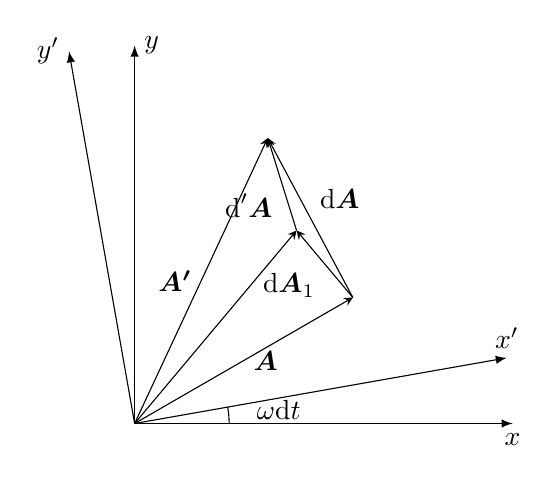
\begin{tikzpicture}[scale=0.8]
            \draw[-latex] (0,0) -- (6,0);
            \draw[-latex] (0,0) -- (0,6);
            \draw[-latex] (0,0) -- (10:6);
            \draw[-latex] (0,0) -- (100:6);
            \draw (1.5,0) arc (0:10:1.5);
            \draw[-stealth] (0,0) -- (30:4);
            \draw[-stealth] (0,0) -- (50:4);
            \draw[-stealth] (30:4) -- (50:4) node [midway, below left] {$\D \boldsymbol{A}_1$};
            \draw[-stealth] (0,0) -- (65:5);
            \draw[-stealth] (50:4) -- (65:5) node [midway, below left] {$\D'\boldsymbol{A}$};
            \draw[-stealth] (30:4) -- (65:5) node [midway, above right] {$\D \boldsymbol{A}$};
            \node[anchor=north] (x-axis) at (6,0) {$x$};
            \node[anchor=west] (y-axis) at (0,6) {$y$};
            \node[anchor=south] (x'-axis) at (10:6) {$x'$};
            \node[anchor=east] (y'-axis) at (100:6) {$y'$};
            \node[anchor=west] (angle1) at (7:1.8) {$\omega \D t$};
            \node at (30:2) [right] {$\boldsymbol{A}$};
            \node at (65:2.5) [left] {$\boldsymbol{A'}$};
        \end{tikzpicture}
        \caption{地面坐标系}
    \end{subfigure}
    \begin{subfigure}{.48\textwidth}
        \centering
        \begin{tikzpicture}[scale=0.8]
            \draw [-latex] (0,0) -- (6,0);
            \draw [-latex] (0,0) -- (0,6);
            \draw [-stealth] (0,0) -- (30:4) node [midway, below right] {$\boldsymbol{A}$};
            \draw [-stealth] (0,0) -- (45:5) node [midway, above left] {$\boldsymbol{A'}$};
            \draw [-stealth] (30:4) -- (45:5) node [midway, right] {$\boldsymbol{\D' \boldsymbol{A}}$};
            \node [anchor = north] (x-axis) at (6,0) {$x'$};
            \node [anchor = east] (y-axis) at (0,6) {$y'$};
        \end{tikzpicture}
        \caption{旋转参考系}
    \end{subfigure}
    \caption{旋转参考系示意}
\end{figure}

如上图,一个矢量 $\boldsymbol{A}$ 在无穷小时间微元内的变化量 $\D \boldsymbol{A}$ 可拆为两个部分: $\D \boldsymbol{A}_1$ 和 $\D' \boldsymbol{A}$.前者是旋转参考系给矢量 $A$ 的一个牵连的变化量,有 $\D \boldsymbol{A}_1 = \omega \times \boldsymbol{A} \D t$.后者是旋转参考系下,$A$ 的"相对"变化量.这是我们让矢量 $A$ 对时间求导,则我们有
\[\derivative{A}{t} = \frac{\D' \boldsymbol{A}}{\D' t} + \omega\times \boldsymbol{A}\]

\chapter{刚体力学}

对于一般刚体的角动量计算,我们会先取惯量主轴,然后将刚体的角速度分解到个主轴方向上,计算沿着各主轴方向的角动量,再合成便是角动量矢量.

下面我们解释一下上面这段话.一个运动的刚体,在无穷小时间微元内,刚体上任意一点的运动可视作为:质心的平动 $\D \boldsymbol{R}$,和绕质心转动无穷小角度 $\D \boldsymbol{\phi} \times \boldsymbol{r}$,即
\[\D \tau = \D \boldsymbol{R} + \D \boldsymbol{\phi} \times \boldsymbol{r}\]
将上式同时对时间求导,即
\[\boldsymbol{v} = \boldsymbol{V} + \boldsymbol{\omega} \times \boldsymbol{r}\]

\part{电磁学}

\chapter{静电学}

\section{库仑定律,高斯定律和矢量场论基础}

\subsection{库仑定律}

首先,静电学的第一条定律是库仑定律,是库仑由扭秤实验测得.其特征是静电力符合平方反比的规律.

\begin{law}
    空间中两个点电荷,电荷量分别为 $q_1,q_2$,则两个点电荷之间的相互作用力为
    \begin{equation}
        \boldsymbol{F} = k \frac{q_1q_2}{r^2} \boldsymbol{\hat{r}}
    \end{equation}
    这条定律被称为\textbf{库仑定律}.式中 $k$ 被称为静电力常量,其值约为 \SI{8.99 E 9}{\newton\square\meter\per\square\coulomb}.
\end{law}

库仑定律中的静电力常量 $k$ 有时还会改写成 $\dfrac{1}{4\pi\vp}$ ,其中 $\vp$ 称为真空介电常数,其值约为 \SI{8.85E-12}{\square\coulomb\per\newton\per\square\meter}.

由库仑定律,我们可以发现,如果空间中有一个点电荷 $Q$ 且它固定不动,那么在这个点电荷周围空间内某一点若再放一个试探点电荷 $q$,这一试探电荷所受到的库仑力与试探点电荷的电荷量成正比.由于电荷量是一个标量,因此我们可以很容易的定义电场.

\begin{definition}
    空间中某点的电场强度,简称电场,定义为在该点放入一个试探电荷 $q_0$,其所受力与试探电荷带电量的比值,即:
    \begin{equation}
        \boldsymbol{E} = \frac{\boldsymbol{F}}{q_0}
    \end{equation}
    特别地,当空间中电场为点电荷电场时,电场强度为
    \[\boldsymbol{E} = \frac{1}{4\pi\vp}\frac{Q}{r_Q^2}\boldsymbol{\hat{r_Q}}\]
\end{definition}

电场强度还满足叠加原理.

\begin{principle}
    空间中某一点的电场强度,等于这一点周围所有电荷对这一点产生的电场强度的矢量和,即:
    \begin{equation}
        \boldsymbol{E}(\boldsymbol{r})\xlongequal{\boldsymbol{r'}:=\boldsymbol{r}-\boldsymbol{r_i}}\sum_i \frac{1}{4\pi\vp}\frac{q_i}{\boldsymbol{r'}^2}\boldsymbol{\hat{r'}}
    \end{equation}
\end{principle}

需要注意几点:

以上的公式都是对于离散的点电荷分布模型说明的.实际上大部分情况下计算的都是连续电荷分布,如体电荷分布,面电荷分布,线电荷分布等等.但是,对于每一个微元(体积元,面元或线元),由于其形状微小,可以将其看做一个电量很少的点电荷,并使用库仑定律和电场强度叠加原理计算某一点的电场强度,从而(1.2)式和(1.3)式需要合并并改写为
\begin{align*}
    \boldsymbol{E}(\boldsymbol{r})&=\iiint_V \frac{1}{4\pi\vp} \frac{\rho_e\D V}{\boldsymbol{r'}^2}\boldsymbol{\hat{r'}} \\
    &=\iint_S \frac{1}{4\pi\vp} \frac{\sigma_e\D S}{\boldsymbol{r'}^2}\boldsymbol{\hat{r'}} \\
    &=\int_l \frac{1}{4\pi\vp} \frac{\lambda_e\D l}{\boldsymbol{r'}^2}\boldsymbol{\hat{r'}} \\
\end{align*}

\subsection{电场中的高斯定理}

下面我们介绍电场中的高斯定理.

\begin{theorem}
    在空间中任取一个闭合面 $S$,并定义电通量为
    \begin{equation}
        \Phi_e=\iint_S \boldsymbol{E} \cdot \D \boldsymbol{s}
    \end{equation}
    其中 $\D \boldsymbol{s}$ 是面积微元,以向外为正方向.则我们有
    \begin{equation}
        \Phi_e=\iint_S \boldsymbol{E} \cdot \D \boldsymbol{s}=\frac{q_S}{\vp}
    \end{equation}
    上式中 $q_S$ 是闭合曲面 $S$ 内的电荷量,而这一个式子便是\textbf{电场中的高斯定理}.
\end{theorem}

接下来我们对这一个定理进行证明.

\begin{proof}
    首先考虑闭合曲面 $S$ 内一点电荷(或电荷元)的情况,这两个模型均可以视作点电荷.因此
    \[\Phi_e = \varoiint_S \frac{1}{4\pi\vp} \frac{q}{r^2} \D \boldsymbol{s} \cos \theta = \varoiint_S \frac{q}{4\pi\vp} \D \Omega = \frac{q}{\vp}\]
    其中 $\Omega$ 为立体角.注意到上式结果跟电荷在闭合曲面 $S$ 中的位置无关,因此由电场的矢量叠加原理,我们可以有
    \[\Phi_e = \frac{q_{in}}{\vp}\]
    
    接着,我们考虑 $S$ 外的电荷,不难发现此时立体角的加和变为了0,因此闭合曲面 $S$ 外的电荷对电通量大小无贡献.

    综上,电场中的高斯定理得证.
\end{proof}

乍一看,高斯定理和库仑定律没有本质区别,看起来是可以等价的两个说法.但实际上,库仑定律研究的力表现出的是一种超距作用:不需要时间就可以传播的相互作用.而高斯定理不一样,它研究的是电场.场的概念确定了电磁相互作用的传播是需要一定时间的.如果库仑定律是完全正确的,那么就会出现违反因果律的现象,即可以通过合适的参考系变换来做到在电磁相互作用改变之前得知电场的改变.这显然是不可能的.

上面的电场中的高斯定理并不是高斯定理本来的形式,它是由麦克斯韦从矢量场论中的数学上的高斯定理移植的.接下来我们就需要介绍矢量分析的基础内容.

\subsection{矢量分析基础}

我们需要引入三个概念:梯度,散度,旋度.

\subsubsection{梯度}

\begin{definition}
    首先是梯度.梯度的定义为:沿线元 $\D \boldsymbol{l}$ ,标量场 $\varphi(x,y,z)$ 的数值改变为 $\D \varphi$.则 $\derivative{\varphi}{l}$ 称为 $\varphi$ 沿 $\D \boldsymbol{l}$ 方向的分量,即
    \[(\grad \varphi)_l = \nabla \varphi = \derivative{\varphi}{l}\]
\end{definition}

这里我们考虑三维空间的曲线坐标系.即空间中某一点的坐标可以表示为 $(u_1,u_2,u_3)$,且沿这三个方向的基矢分别为 $\boldsymbol{e_1},\boldsymbol{e_2},\boldsymbol{e_3}$,线元长度与坐标微分的关系分别是 $\D l_1=h_1\D u_1,\D l_2=h_2\D u_2,\D l_3=h_3\D u_3$,则不难发现,梯度可以写为
\begin{equation}
    \nabla \varphi = \boldsymbol{e_1} \pd{\varphi}{l_1} + \boldsymbol{e_2} \pd{\varphi}{l_2} + \boldsymbol{e_3} \pd{\varphi}{l_3} = \boldsymbol{e_1} \frac{1}{h_1} \pd{\varphi}{u_1} + \boldsymbol{e_2} \frac{1}{h_2} \pd{\varphi}{u_2} + \boldsymbol{e_3} \frac{1}{h_3} \pd{\varphi}{u_3}
\end{equation}
式中 $h_1,h_2,h_3$ 称为\textbf{拉梅系数}.

\subsubsection{散度}

\begin{definition}
    接下来是散度的定义.散度被定义为,某一点处附近体积元的通量与体积元体积的比值的极限:
    \[\divergence \boldsymbol{A}=\nabla \cdot \boldsymbol{A} = \lim_{\Delta V\to 0} \frac{\displaystyle \varoiint_S \boldsymbol{A} \cdot \D \boldsymbol{s}}{\Delta V}\]
    上式中, $\D \boldsymbol{s}$ 取向外为正方向
\end{definition}

对于一个正交曲线坐标系,我们先画出一个体积微元:

\begin{figure}[htbp]
    \centering
    \begin{tikzpicture}[scale=3]
        \draw [-latex] (0,0,0) -- (1.5,0,0);
        \draw [-latex] (0,0,0) -- (0,1.5,0);
        \draw [-latex] (0,0,0) -- (0,0,1.5);
        \draw (1,0,0) -- (1,1,0) -- (1,1,1) -- (1,0,1) -- (0,0,1);
        \draw (1,0,0) -- (1,0,1);
        \draw (0,0,1) -- (0,1,1) -- (0,1,0) -- (1,1,0);
        \draw (0,1,1) -- (1,1,1);
        \node [anchor=south] (u1) at (1.5,0,0) {$u_1$};
        \node [anchor=east] (u2) at (0,1.5,0) {$u_2$};
        \node [anchor=west] (u3) at (0,0,1.5) {$u_3$};
        \node [anchor=south] (dl1) at (0.5,0,0) {$\D l_1$};
        \node [anchor=west] (dl2) at (0,0.5,0) {$\D l_2$};
        \node [anchor=south] (dl3) at (0,0,0.5) {$\D l_3$};
    \end{tikzpicture}
    \caption{正交曲线坐标系体积微元}
\end{figure}

我们可以计算其通量.通过平行于 $u_2u_3$ 两平面的通量为 $\Phi_1=A_1(u_1 + \D l_1) \D l_2'\D l_3'-A_1(u_1) \D l_2\D l_3$,同理我们可以得到其余两个式子,并对其加和有
\begin{align*}
    \Phi &= \Phi_1+\Phi_2+\Phi_3 \\
    &= A_1(u_1 + \D l_1) \D l_2'\D l_3'-A_1(u_1) \D l_2\D l_3 \\
    &+ A_2(u_2 + \D l_2) \D l_1'\D l_3'-A_2(u_2) \D l_1\D l_3 \\
    &+ A_3(u_3 + \D l_3) \D l_1'\D l_2'-A_3(u_3) \D l_1\D l_2 \\
    &= \D (A_1h_2h_3) \D u_2 \D u_3 + \D (A_2h_1h_3) \D u_1 \D u_3 + \D (A_3h_1h_2) \D u_1 \D u_2
\end{align*}
根据散度的定义,我们除以体积元 $\Delta V = h_1h_2h_3\D l_1 \D l_2 \D l_3$,则有
\begin{equation}
    \nabla \cdot \boldsymbol{A} = \frac{1}{h_1h_2h_3} \left(\pd{A_1h_2h_3}{u_1} + \pd{A_2h_1h_3}{u_2} + \pd{A_3h_1h_2}{u_3}\right)
\end{equation}
这便是正交三维坐标系下的散度公式.

\subsubsection{旋度}

\begin{definition}
    接下来是旋度.在某一点附近取一个闭合回路,并以该回路为边界取一个面元.面元矢量 $\D \boldsymbol{s}$ 方向与闭合回路的绕行方向满足右手定则关系.那么,矢量场沿该闭合回路的积分与 $\D \boldsymbol{S}$ 的比值的极限,称为该矢量场在该点处旋度沿面元法向的分量,即:
    \[\left(\curl \boldsymbol{f}\right)_n = \left(\nabla \times \boldsymbol{f}\right) = \lim_{\D s\to 0} \frac{\displaystyle \oint_l \boldsymbol{f} \cdot \D \boldsymbol{l}}{\D S}\]
\end{definition}

对于正交三维曲线坐标系 $u_1u_2u_3$,我们可以以某一点为起点,分别在 $u_1u_2,u_1u_3,u_2u_3$ 三个平面上取三个矩形回路,从而计算矢量场旋度的三个分量.我们先计算沿 $u_1$ 方向的分量.
\begin{align*}
    &\left(\nabla \times \boldsymbol{f}\right)_1 \\
    = &\frac{1}{h_2h_3\D u_2\D u_3} \left(h_2\D u_2 f_2(u_2) - h_2'\D u_2 f_2(u_2 +\D u_2) + h_3'\D u_3 f_3(u_3 +\D u_3) - h_3\D u_3 f_3(u_3)\right) \\
    = & \frac{1}{h_2h_3}\left(\downpd{f_3h_3}{u_2} - \downpd{f_2 h_2}{u_3}\right)
\end{align*}
类似地,我们还可以写出旋度沿剩下两个方向的分量,即:
\begin{align*}
    & (\nabla \times \boldsymbol{f})_2 = \frac{1}{h_1h_3} \left( \downpd{f_1h_1}{u_3} - \downpd{f_3h_3}{u_1}\right) \\
    & (\nabla \times \boldsymbol{f})_3 = \frac{1}{h_1h_2} \left( \downpd{f_2h_2}{u_1} - \downpd{f_1h_1}{u_2}\right)
\end{align*}
组合起来,则我们有:
\begin{align}
    \nabla \times \boldsymbol{f} = &\frac{1}{h_2h_3}\left(\downpd{f_3h_3}{u_2} - \downpd{f_2 h_2}{u_3}\right) \boldsymbol{e_1} \notag \\ 
    + &\frac{1}{h_1h_3} \left( \downpd{f_1h_1}{u_3} - \downpd{f_3h_3}{u_1}\right)\boldsymbol{e_2} \notag \\
    + &\frac{1}{h_1h_2} \left( \downpd{f_2h_2}{u_1} - \downpd{f_1h_1}{u_2}\right)\boldsymbol{e_3}
\end{align}

\subsubsection{拉普拉斯算符}

\begin{definition}
    最后是拉普拉斯算符,其定义为一个标量场的梯度的散度,即:
    \[\nabla \cdot \nabla \varphi \equiv \nabla^2 \varphi\]
\end{definition}

当然,拉普拉斯算符也可以作用在矢量场上,这将在后面的并矢中提到.这里我们先写出标量场的拉普拉斯算符,只需要按照定义将上面的定义式表示出来即可,书写过程已经是无意义的,这里直接给出答案:
\begin{equation}
    \nabla^2 \psi = \frac{1}{h_1h_2h_3} \left(\downpd{\frac{h_2h_3}{h_1} \pd{\psi}{u_1}}{u_1} + \downpd{\frac{h_1h_3}{h_2} \pd{\psi}{u_2}}{u_2} + \downpd{\frac{h_1h_2}{h_3} \pd{\psi}{u_3}}{u_3}\right)
\end{equation}

\subsubsection{公式总结}

这里我们给出一些常用坐标系下的梯度,散度,旋度和拉普拉斯:

\paragraph{直角坐标系}

\begin{align}
    \nabla \psi &= \pd{\psi}{x}\boldsymbol{\hat{x}} + \pd{\psi}{y}\boldsymbol{\hat{y}} + \pd{\psi}{z}\boldsymbol{\hat{z}} \\
    \nabla \cdot \boldsymbol{f} &= \pd{f_x}{x} + \pd{f_y}{y} + \pd{f_z}{z} \\
    \nabla \times \boldsymbol{f} &=
    \begin{vmatrix}
        \boldsymbol{\hat{x}} & \boldsymbol{\hat{y}} & \boldsymbol{\hat{z}} \\
        \displaystyle \pdn{x} & \displaystyle \pdn{y} & \displaystyle \pdn{z} \\
        f_x & f_y & f_z
    \end{vmatrix} \notag \\
    &= \left(\pd{f_z}{y} - \pd{f_y}{z}\right)\boldsymbol{\hat{x}} + \left(\pd{f_x}{z}-\pd{f_z}{x}\right)\boldsymbol{\hat{y}} + \left(\pd{f_y}{x}-\pd{f_x}{y}\right)\boldsymbol{\hat{z}} 
\end{align}
值得一提的是,从直角坐标系中可以看出 $\nabla$ 这一算符的矢量性,点乘和叉乘的规则都符合了.事实上,在球坐标系和柱坐标系中也是符合的,但是在这两个坐标系中,对某些基矢求偏导数可能会出现一些新的项,导致结果与叉乘不甚相似. 非直角坐标系下的旋度也可以用三阶行列式表示,但不会像直角坐标系那样如此简单,下面我们会一一给出,以方便记诵.

\paragraph{柱坐标系}
\begin{align}
    \nabla \psi &= \boldsymbol{\hat{\rho}} \pd{\psi}{\rho} + \bv{\theta} \frac{1}{r} \pd{\psi}{\theta} + \bv{z} \pd{\psi}{z} \\
    \nabla \cdot \boldsymbol{A} &= \frac{1}{\rho}\downpd{\rho A_\rho}{\rho} + \frac{1}{\rho}\pd{A_\theta}{\theta} + \pd{A_z}{z} \\
    \nabla \times \boldsymbol{A} &= \left(\frac{1}{\rho} \pd{A_z}{\theta} - \pd{A_\theta}{z}\right)\bv{\rho} + \left(\pd{A_\rho}{z} - \pd{A_z}{\rho}\right)\bv{\theta} + \frac{1}{\rho}\left(\downpd{\rho A_\theta}{\rho} - \pd{A_\rho}{\theta}\right)\bv{z}
\end{align}

旋度的行列式表示方法为:
\begin{equation}
    \nabla \times \boldsymbol{A} = \frac{1}{\rho}
    \begin{vmatrix}
        \bv{\rho} & \rho\bv{\theta} & \bv{z} \\
        \pd{}{\rho} & \pd{}{\theta} & \pd{}{z} \\
        A_\rho & \rho A_\theta & A_z
    \end{vmatrix}
\end{equation}

\paragraph{球坐标系}
\begin{align}
    \nabla \psi &= \bv{r} \pd{\psi}{r} + \bv{\theta} \frac{1}{r} \pd{\psi}{\theta} + \bv{\phi} \frac{1}{r\sin \theta} \pd{\psi}{\phi}\\
    \nabla \cdot \boldsymbol{A} &= \frac{1}{r^2}\downpd{r^2A_r}{r} + \frac{1}{r\sin \theta}\downpd{f_\theta \sin \theta}{\theta} + \frac{1}{r\sin \theta}\downpd{f_\phi}{\phi} \\
    \nabla \times \boldsymbol{A} &= \frac{1}{r\sin \theta}\left( \downpd{\sin \theta A_\phi}{\theta} - \pd{A_\theta}{\phi} \right) \bv{r} + \frac{1}{r} \left( \frac{1}{\sin \theta} \pd{A_r}{\phi} - \downpd{rA_\phi}{r}\right) \bv{\theta} \notag \\
    &+ \frac{1}{r}\left( \downpd{rA_\theta}{r} - \pd{A_r}{\theta} \right) \bv{\phi}
\end{align}

旋度的行列式表示方法为:
\begin{equation}
    \nabla \times \boldsymbol{A} = \frac{1}{r^2 \sin \theta}
    \begin{vmatrix}
        \bv{r} & r\bv{\theta} & r\sin \theta \bv{\phi} \\
        \pd{}{r} & \pd{}{\theta} & \pd{}{\phi} \\
        A_r &  rA_\theta & r\sin \theta A_\phi
    \end{vmatrix}
\end{equation}

\part{数学物理方法}

\chapter{解析函数与复变函数}

\section{复数的定义,基本概念}

首先我们要引进复数,原因是有些方程不存在实数解.举个最简单的实系数方程:
\[x^2+1=0\]
这个方程式没有实数解的,这是因为对于任意实数都有 $x^2\geqslant0$,这样看上去十分难受,为了让这个方程也有解,数学家门定义了一个新的数.

\begin{definition}
    如果一个数 $x$ 满足 $x^2=-1$,那么我们称这个数 $x$ 为虚数单位 $i$,即
    \begin{equation}
        i^2=-1
        \label{def of i}
    \end{equation}
\end{definition}

其符号来由,是因为这个数并非"真正的"数,因此称其为"虚数",而称原来所谓的"真正的数"为"实数".虚数在英文中是 Imaginary number,即想象出来的数,和"虚数"的意义相似,因此用符号来表示虚数单位 $i$.

首先我们需要定义复数

\begin{definition}
    假设我们有一个二元有序\textbf{实数对} $(x,y)$,那么我们可以定义这样一个数 $z$ 满足 $z=x+iy$,其中 $i$ 为 (\ref{def of i}) 中定义的虚数单位.此时,我们称 $z$ 为一个复数,其中 $x$ 为复数 $z$ 的实部,记作 $\operatorname{Re} z=x$.类似地,我们称 $y$ 为复数 $z$ 的虚部,记作 $\operatorname{Im}z = y$.
\end{definition}

接下来我们定义复共轭.

\begin{definition}
    如果有一个复数 $z=x+iy$,那么我们定义它的复共轭为
    \begin{equation}
        z^* = \bar z \equiv x-iy
    \end{equation}
    一般我们采用前面那种写法表示复共轭.
\end{definition}

我们还需要定义复数中的相等.
\begin{definition}
    有两个复数 $z_1,z_2$,分别满足 $z_1=x_1+iy_1,z_2=x_2+iy_2$,如果有 $x_1=x_2,y_1=y_2$,则我们称两个复数相等,记作 $z_1=z_2$
\end{definition}

需要注意的是,虽然我们有复数"相等"的概念,但是并不能定义复数的比大小.可以试着定义一种比较两个复数大小的方案,总可以找到悖论.

\section{复数的其他表示方法}

前面我们介绍了复数的定义,以及代数表示.代数表示的缺点是比较抽象,优点就是写的时候比较方便.为了弥补代数表示的缺点,我们为复数寻找了一种几何表示,其优点是非常具象,但是记录的时候却比较复杂.

\begin{figure}[htbp]
    \centering
    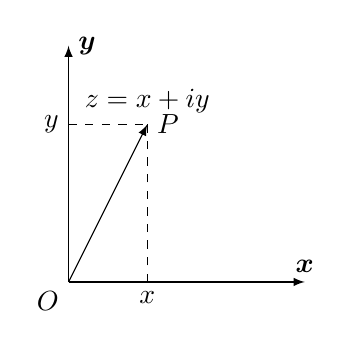
\begin{tikzpicture}
        \draw [-latex] (0,0) -- (0,3);
        \draw [-latex] (0,0) -- (3,0);
        \node at (0,3) [right] {$\boldsymbol{y}$};
        \node at (3,0) [above] {$\boldsymbol{x}$};
        \node at (0,0) [below left] {$O$};
        \draw [-latex] (0,0) -- (1,2);
        \node (P) at (1,2) [right] {$P$};
        \draw [dashed] (0,2) -- (1,2);
        \draw [dashed] (1,0) -- (1,2);
        \node at (1,0) [below] {$x$};
        \node at (0,2) [left] {$y$};
        \node at (1,2.3) {$z=x+iy$};
    \end{tikzpicture}
    \caption{复数的几何表示和矢量表示}
    \label{Fig:复数的几何表示和矢量表示}
\end{figure}

几何表示中,复数 $z=x+iy$ 就是图 \ref{Fig:复数的几何表示和矢量表示} 中的 $P$ 点,而矢量表示就是图 \ref{Fig:复数的几何表示和矢量表示} 中的 $\overrightarrow{OP}$.

图 \ref{Fig:复数的几何表示和矢量表示} 中,建立的 $x-y$ 平面并非一般的平面直角坐标系,我们称其为复平面.只有在说明"建立复平面"后,才能用几何表示或矢量表示说明图中某一点或矢量表示的复数.否则,我们的讨论仅限于之前建立的实数理论中.

这里稍微提一嘴,在直观的几何表示和矢量表示中,复数"相等"的定义方式也是显而易见的.对于几何表示,就是两个点重合,对于矢量表示,就是两个矢量相等,也就是两个矢量大小相等,方向相反.

以上是复数在平面直角坐标系中的表示方法,显然我们可以将这个平面直角坐标系更换为平面极坐标系.下面给出复数的极坐标表示.

\begin{definition}
    我们称在复平面中,一个复数 $z$ 所表示的矢量长度为这个复数的模,记作 $|z|$.为了方便,这里我们用 $r$ 表示.
\end{definition}
\begin{definition}
    如果我们用极坐标系复数 $z$ 所表示一个点 $P$ 的位置,需要两个坐标 $(r,\theta)$,我们称 $\theta$ 为复数 $z$ 的辐角.记作 $\operatorname{arg} z$.
\end{definition}
\begin{definition}
    由于 $r\neq0$ 时,辐角可以差 $2n\pi(n=0,1,2,\cdots)$,则我们定义在 $(-\pi,\pi]$ 的辐角称为复数 $z$ 的辐角主值,记作 $\operatorname{Arg} z$
\end{definition}

著名的 Euler 公式给出了复数的指数表示方法.
\begin{theorem}[Euler 公式]
    对于函数 $f(\theta)=e^{i\theta}$,它的值满足:
    \begin{equation}
        f(\theta) = e^{i\theta} = \cos \theta + i\sin \theta
    \end{equation}
    这就是著名的 Euler 公式.
\end{theorem}

这个定理的证明需要用到 Taylor 展开,当然这并不困难.
\begin{proof}
    我们知道,函数 $g(x) = e^x$ 在 0 附近出的泰勒展开为:
    \[
    g(x) = e^x = \sum _{m=0}^{+\infty} \frac{x^m}{m!}
    \]
    这个时候,我们代入 $x=i\theta$,则有:
    \begin{align*}
        f(\theta) = g(i\theta) &= \sum_{m=0}^{+\infty}\frac{x^m}{m^!} \\
        &= 1 + i\frac{x}{1!} - \frac{x^2}{2!} -i\frac{x^3}{3!} +\frac{x^4}{4!} +i\frac{x^5}{5!} -\cdots
    \end{align*}
    注意到两个三角函数的 Taylor 展开分别是:
    \begin{align*}
        &\cos\theta = 1 - \frac{x^2}{2!} + \frac{x^4}{4!} -\cdots \\
        &\sin\theta = \frac{x}{1!} - \frac{x^3}{3!} + \frac{x^5}{5!} -\cdots
    \end{align*}
    因此,我们有
    \[
    e^{i\theta} = \cos\theta + i\sin\theta
    \]
    Euler 公式得证.
\end{proof}

我们还有一种表示方法:球面表示.我们过复平面原点作一球面鱼复平面相切,切点为该球面的南极点,并记这个球面的北极点为 $N$.对任意在复平面上的一点 $z$,连接该点与 $N$ 交球面于一点 $\zeta$,显然 $z$ 与 $\zeta$ 一一对应,$\zeta$ 即为复数 $z$ 的球面表示.北极点对应复平面上的无穷远点.需要注意的是,无穷远点的辐角是没有定义的.

当然,这种球面表示方法非常高级,在这一阶段我们并不常用,这里只是略提一句.

\section{复数的代数运算}

再说一遍:\textbf{复数不能比较大小!}但是我们知道,复数的模是一个实数,是可以比较大小的.接下来我们定义复数的加减法.

\begin{definition}
    两个复数 $z_1=x_1+iy_1,z_2=x_2+iy_2$,定义加法为:
    \begin{equation}
        z_1\pm z_2=(x_1\pm x_2) + i(y_1\pm y_2)
    \end{equation}
    不难验证,复数的加法满足交换律与结合律.这里不给出证明.
\end{definition}

加减法的几何意义,就是在复平面上两个矢量相加的平行四边形法则.当然由三角形两边之和大于第三边,两边之差小于第三边,我们可以列出以下的不等式
\begin{align}
    |z_1+z_2| \leqslant |z_1| + |z_2| \label{equ:inequality 1}\\
    |z_1-z_2| \geqslant |z_1| - |z_2| \label{equ:inequailty 2}
\end{align}
如果你愿意,你也可以在(\ref{equ:inequailty 2})式右边再加上绝对值符号,结论仍然成立.

我们还需要定义复数的乘除法运算.我们先定义乘法,显然这比较容易:
\begin{definition}
    如果有两个复数$z_1,z_2$,满足:
    \begin{align*}
        &z_1 = x_1 + iy_1 = r_1e^{i\theta_1} \\
        &z_2 = x_2 + iy_2 = r_2e^{i\theta_2} \\
    \end{align*}
    则它们的乘积定义为:
    \begin{align}
        z_1z_2 &= (x_1+iy_1)(x_2+iy_2) \nonumber \\
        &= (x_1x_2-y_1y_2) + i(x_1y_2+x_2y_1) \label{equ:def of product 1}\\
        &= r_1r_2e^{i(\theta_1+\theta_2)} \label{equ:def of product 2}
    \end{align}
    同样不难验证复数的乘法仍然满足分配律,结合律和交换律.
\end{definition}

复数的乘法的几何意义为:将原两复数的模的乘积作为新的复数的模,将两复数的辐角相加作为新的复数的辐角.

然后我们定义复数的除法,其几何意义和乘法类似.如果我们要计算 $z=z_1/z_2$ ,那么 $z$ 的模长为 $|z_1|/|z_2|$,辐角为 $\operatorname{Arg}z_1-\operatorname{Arg}z_2$(这里再取一次辐角主值).复数的除法的代数定义如下:

\begin{definition}
    如果复数 $z_1=x_1+iy_1,z_2=x_2+iy_2$,则
    \begin{align}
        \frac{z_1}{z_2} = \frac{x_1+iy_1}{x_2+iy_2} &= \frac{(x_2-iy_2)(x_1+iy_1)}{(x_1+iy_1)(x_1-iy_1)} \nonumber \\
        &= \frac{x_1x_2+y_1y_2}{x_2^2+y_2^2} + i\frac{(x_2y_1-x_1y_2)}{x_2^2+y_2^2}
        \label{equ:def of division}
    \end{align}
\end{definition}

我们还要定义复数的乘方.

\begin{definition}
    对于复数 $z=re^{i\theta}$,其 $n$ 次方被定义为:
    \begin{align}
        z^n &= r^ne^{in\theta} \label{equ:def of pow 1} \\
        &= r^n(\cos n\theta + i\sin n\theta) \label{equ:def of pow 2}\\
        &= r^n(\cos\theta +i\sin\theta)^n \label{equ:def of pow 3}
    \end{align}
\end{definition}

从(\ref{equ:def of pow 2})式和(\ref{equ:def of pow 3})式可以看出这样的关系:
\begin{equation}
    (\cos\theta+i\sin\theta)^n = \cos n\theta +i\sin n\theta
    \label{equ:Demoivre}
\end{equation}
(\ref{equ:Demoivre})式称为 Demoivre 定理.

\section{复数序列的极限}

这一节纯粹是为下面一节做铺垫用的,毕竟我们在学函数极限的时候就是先学序列的极限,再引入到函数的极限的.下面先定义复数序列,这很好理解,由字面意思就可以理解:

\begin{definition}
    复数序列的定义为,按一定顺序排列的复数,记为 $\{z_n\}$,其中 $z_n=x_n+iy_n,n=1,2,3,\cdots$.
\end{definition}

我们还要定义一些其他的东西,第一个是聚点.
\begin{definition}
    对于 $\forall \epsilon>0$,都 $\exists$ 无穷多个 $z_n$ 满足 $|z-z_n| < \epsilon$,那么我们称 $z$ 为复数序列 $\{z_n\}$ 的一个聚点.
\end{definition}
接下来是复数序列的极限:
\begin{definition}
    对于 $\forall \epsilon>0$,都 $\exists N(\epsilon) > 0$ 使得当 $n>N$ 恒有 $|z-z_n| < \epsilon$,则称 $z$ 为复数序列 $\{z_n\}$ 的极限.记作
    \[
        \lim_{n\to\infty}z_n=z
    \]
    这很像一般序列极限中的 $\epsilon-N$ 语言,或者说,这是复数序列版本的 $\epsilon-N$语言.
\end{definition}

一个序列可以有多个聚点.但是当一个序列的极限存在时,极限是序列唯一的聚点.对于更特殊的实数序列,最大的聚点称为序列的上极限,记为 $\displaystyle\varlimsup_{n\to\infty}  z_n$;最小的聚点称为序列的下极限,记为:$\displaystyle\varliminf _{n\to\infty} z_n$

当然,我们也有和一般序列极限类似的 Cauchy 判据.
\begin{theorem}
    一个复数序列极限存在的充要条件是,$\forall\epsilon > 0,\exists N(\epsilon) > 0$,使得 $n>N$ 时,$\forall p\in \mathbb{N}^{*}$,恒有 $|z_{n+p}-z_n|<\epsilon$.
\end{theorem}

我们也需要一个极限趋于无穷的定义
\begin{definition}
    $\forall M>0,\exists N(M)>0$,使得 $n>N$ 时,恒有 $|z_n|>M$,记为 $\displaystyle \lim_{n\to\infty} z_n=\infty$
\end{definition}

\section{复变函数,复变函数的极限与连续}

首先,我们要引入区域的概念.函数的概念推广到复数数域,自变量使复数,取值范围在复平面的某个区域,类似于二元函数,但是异于二元函数.下面引入一些概念:

\begin{definition}
    复平面上任意一些点的集合成为点集.
\end{definition}

\begin{definition}
    点 $z_0$ 的 $\epsilon$ 邻域是指满足 $|z-z_0| < \epsilon$ 的点集,以 $z_0$ 为中心,$\epsilon$ 为半径的圆内.
\end{definition}

\begin{definition}[去心邻域]
    又称无心领域,就是指满足 $0<|z-z_0|<\epsilon$的点集.
\end{definition}

\begin{definition}[内点]
    是指点集 $S$ 中可以找到该店的一个邻域,使得该邻域的点都属于点集 $S$.
\end{definition}

\begin{definition}[开区域]
    满足以下两个条件的区域称为开区域:
    \begin{enumerate}
        \item 每一点都是内点.
        \item 点集中的任意两点均可用一条属于该点集的点构成的曲线或折线相连.
    \end{enumerate}
\end{definition}

\begin{definition}[边界点]
    不属于开区域 $D$,但其任一邻域均包含属于 $D$ 与不属于 $D$ 的点.
\end{definition}

\begin{definition}
    开区域加上边界点,记为 $\overline{D}$
\end{definition}

\begin{definition}[全平面]
    不包括无穷远点的整个复平面,也称复平面.
\end{definition}

\begin{definition}[闭平面]
    包括无穷远点的整个复平面,也称扩充复平面.
\end{definition}

\begin{definition}[单连通区域]
    边界为一条简单闭合曲线构成的区域.
\end{definition}

\begin{definition}[复连通区域]
    边界由多于一条闭合曲线构成.
\end{definition}

以下是几点补充:
\begin{enumerate}
    \item 通常我们用 $D$ 来表示开区域,$\overline{D}$ 来表示闭区域,$\overline{D}=D+C$,$C$ 为边界点.
    \item 对复平面,无穷远点是它的边界点,对扩充复平面,无穷远点属于内点.
    \item 扩充复平面是唯一的一个无边界点的区域;
    \item 有限远点 $z_0$ 的 $\delta$ 邻域为满足 $|z-z_0|<\delta$ 的所有点,而无穷远点的 $\delta$ 邻域为满足 $|z|>1/\delta$ 的点,即:以远点为中心,$1/\delta$ 为半径圆之外的点集.\footnote{这个定义方式的来源,是一个变换 $w=1/z$,这样在 $z$ 的复平面上,无穷远点对应与 $w$ 的复平面上的原点,在 $w$ 上的 $\delta$ 邻域也就对应到原 $z$ 复平面上的 $|z|>1/\delta$区域.}
    \item 区域边界的正向为,沿着区域的边界走,区域在左手边.
\end{enumerate}

接下来就可以引入复变函数了.
\begin{definition}[复变函数]
    对于复变量在某一个区域取的每一个复数值 $z=x+iy$(或每一对 $(x,y)$ 值),按照一定的规律,有\textbf{一个或多个}复数值 $w=u+iv$ 与之对应,则称 $w$ 是 $z$ 的函数,记为 $w=f(z)$,或
    \[
        w=f(z)=u(x,y)+iv(x,y)
    \]
    这样的函数 $f(z)$ 称为复变函数.
\end{definition}

需要注意的是,复变函数虽然看起来像是两个二元实变函数的有序组合,其许多性质是二元实变函数的推广,但他不仅仅是两个二元实变函数的推广.最显著的特点就是,这里的函数定义规定为\textbf{一个或多个复数值},而实变函数中函数的定义通常是\textbf{有确定的值},也就是一个值而非多个值.举个例子,复变函数中的开根
\[
w=f(z) = \sqrt{z} = z^{1/2} = \sqrt{r}e^{i\left( \frac{\theta}{2} + k\pi \right)},k=0,1,2,\cdots
\]

我们是否可以像实变函数那样规定根式函数只取 $k=0$ 对应的根?不能.若规定只取 $k=0$ 的根,就等价于确定了复变量 $z$ 的辐角,从而使得对复平面上的点,不再让其辐角有 $\pm 2k\pi$ 的自由度.那么在今后做积分时,积分路径沿圆心于原点的原逆时针绕一周回到起点,复变量 $z$ 虽然在复平面上回到了起点,但是辐角增加了 $2\pi$,显然剥夺复变量 $z$ 的辐角有 $\pm 2k\pi$ 这个做法是不合理的.因此,复变函数无法回避多值性.

当然,我们也有另一种理解方式.对实变量的开平方函数,积分只能在实轴上跑, $x<0$ 的区间是不能到达的,相当于规定了不可逾越的边界.因此在规定了 $x=0$ 是不可逾越的边界之后,我们就可以放心地取正根单值函数,也就是算术根.但是对复变函数,如果只取单值函数,会出现不自洽,因此我们也可以通过规定某些不可逾越的边界来使我们的复变函数退化为单值函数.所谓多值函数的割线,整式规定了一条不可逾越的鸿沟,才退化为单值函数的.为此,我们先讨论单值函数,掌握了单值函数后,再接触多值函数.

\begin{definition}[定义域]
    自变量在 $z$ 平面内的取值区域.
\end{definition}

\begin{definition}[值域]
    函数值 $w$ 平面内的取值区域.
\end{definition}

注意到,对于自变量在 $z$ 平面内沿某条曲线 $L$ 变动,函数值在 $w$ 平面内沿另一条曲线 $L'$ 变动.对于单值复变函数,$L$ 与 $L'$ 上的点由 $w=f(z)$ 确定了一一对应关系,这种对应称为从 $z$ 平面到 $w$ 平面的一个映射,这就是复变函数的几何意义.

\begin{definition}[复变函数的极限]
    如果复变函数 $w=f(z)=u(x,y)+iv(x,y)$ 是在 $z_0$ 的一个去心邻域有定义的单值函数,且 $\forall\epsilon>0,\exists\delta(\epsilon)$,使得 $0<|z-z_0|<\delta$ 时,恒有 $|f(z)-w_0|<\epsilon$,则称函数 $f(z)$ 在 $z\to z_0$ 的极限,记为
    \[
    \lim_{z\to z_0}f(z)=w_0
    \]
\end{definition}

从定义可以看出,极限值 $w_0$ 与 $z\to z_0$ 的方式无关,若 $z\to z_0$ 方式不同导致了 $f(z)$ 的极限值不同,则称 $f(z)$ 的极限不存在.这与实变函数的极限定义类似.由于能有极限定义的复变函数一定在此处是单值函数,相当于一对有序的二元实变函数,故极限的各性质是二元实变函数的传承,没有新的特性.因此如果两个复变函数 $f,g$ 在 $z_0$ 处的极限都存在,有:
\begin{align}
    \lim_{z\to z_0}(f\pm g)=\lim_{z\to z_0}f\pm \lim_{z\to z_0}g
    \label{equ:property of lim, plus minus} \\
    \lim_{z\to z_0} fg=\lim_{z\to z_0}f \lim_{z\to z_0}g
    \label{equ:property of lim, product} \\
    \lim_{z\to z_0} \frac{f}{g} = \frac{\displaystyle\lim_{z\to z_0}f}{\displaystyle\lim_{z\to z_0}g},\text{if}\,\lim_{z\to z_0}g\neq 0
    \label{equ:property of lim, division}
\end{align}

\begin{definition}[函数连续]
    如果一个函数在某一点的值等于该点处的极限值,即
    \[
    \lim_{z\to z_0} f(z)=f(z_0)
    \]
    那么我们称这个函数连续.

    当然,我们还有 $\epsilon-\delta$ 定义:函数 $w=f(z)$ 在 $z_0$ 的一个邻域内有定义,且 $\forall\epsilon>0,\exists\delta(\epsilon,z_0)$,使得当 $|z-z_0|<\delta$ 时,有 $|f(z)-f(z_0)|<\epsilon$,则称函数 $w$ 在 $z_0$ 连续.

    更进一步地,如果一个复变函数在区域 $D$ 内的每一点都连续,则称函数 $f(z)$ 在区域 $D$ 内连续.
\end{definition}

注意到,在某点连续的复变函数,在该点的邻域内一定是单值函数,从而它等价于两个二元实变函数,即 $u(x,y)$ 和 $v(x,y)$ 均连续,从而:
\begin{align*}
    \lim_{x\to x_0 \atop y\to y_0}u(x,y)=u(x_0,y_0) \\
    \lim_{x\to x_0 \atop y\to y_0}v(x,y)=v(x_0,y_0)
\end{align*}

\begin{definition}[一致连续]
    函数 $w=f(z)$ 在区域 $D$ 或闭区域 $\overline{D}$ 有定义,$\forall z_0\in D,\epsilon>0,\exists\delta(\epsilon)$,使得当 $|z-z_0|<\delta$ 时,有 $|f(z)-f(z_0)|<\epsilon$,则称 $w=f(z)$ 在该区域 $D$ 内一致连续.

    一致连续的定义也表述为:$\forall\epsilon>0,\exists\delta>0$,使得对区域内满足 $|z_1-z_2|<\delta$ 的任意两点 $z_1,z_2$,恒有 $|f(z_1)-f(z_2)|<\epsilon$.证明非一致连续时常用该定义反证.
\end{definition}

以下是对一致连续的几点说明:
\begin{enumerate}
    \item 连续是对每个点而言,一致连续是对一个区域而言;
    \item 一致连续要求能找到与 $z_0$ 无关的 $\delta$,找到了才能称一致连续,若找不到只能称为连续.
    \item 若函数 $f(z)$ 在一个闭区域 $\overline{D}$ 内连续,则 $f(z)$ 在该闭区域内必然一致连续.
\end{enumerate}

以上性质与二元实变函数完全相同,这是因为一致连续并非复变函数的新概念.

\section{复变函数的导数与 Cauchy-Riemann 条件}

\begin{definition}
    设 $w=f(z)$ 是区域 $D$ 内的单值函数,若在 $D$ 内某点 $z_0$,极限
    \[
    \lim_{z\to z_0}\frac{f(z)-f(z_0)}{z-z_0} = \lim_{\Delta z\to 0} \frac{f(z_0+\Delta z)-f(z)}{\Delta z}
    \]
    存在,则称 $f(z)$ 在 $z_0$处可到,极限值为函数 $f(z)$ 在 $z_0$ 的导数,记为
    \[
    f'(z_0) = \lim_{\Delta z\to 0}\frac{f(z_0+\Delta z)-f(z)}{\Delta z}=\left( \derivative{f(z)}{z} \right)_{z=z_0}
    \]
\end{definition}

可以发现导数其实是变化率的极限,这点与一元实变函数类似.因此,复变函数的一些性质与实变函数类似.

\begin{enumerate}
    \item 如果函数在 $z_0$ 处可到,则函数必在 $z_0$ 点连续.
    \item 实变函数的求导法则可以推广到复变函数.
    \item 无穷远点的导数的计算方式,是比较特别的.需要先进行 $\zeta = 1/z$ 的变换,接着对 $f(z)=f(1/\zeta)$ 进行求导,从而有
    \[
    \left( \derivative{f(z)}{z} \right)_{z=\infty} \xLongrightarrow{z=1/\zeta} \left( \derivative{f(1/\zeta)}{1/\zeta} \right)_{\zeta=0} = -\zeta^2\left( \derivative{f(1/\zeta)}{\zeta} \right)_{\zeta=0}
    \]
    \item 实变函数的导数只需 $\displaystyle\lim_{x\to x_0}\frac{f(x)-f(x_0)}{x-x_0}$ 的左右极限相等,而复变函数则要求无论 $\Delta z$ 以何种方式趋于 0,极限均存在且相等,可见复变函数可导的要求十分苛刻,但其性质更为丰富.
\end{enumerate}

从导数开始,复变函数开始有别于两个有序的二元实变函数.

\begin{definition}
    若函数变化值 $\Delta w=f(z+\Delta z)-f(z)$ 可写成
    \[
        \Delta w=\alpha\Delta z+o(\rho)
    \]
    其中
    \begin{align*}
        &\rho=\left( (\Delta x)^2+(\Delta y)^2 \right)^{1/2} \\
        &\lim_{\Delta z\to 0}\frac{o(\rho)}{\Delta z}=0
    \end{align*}
    那么我们称函数 $w$ 在 $z$ 点可微, $\D w=\alpha\Delta z$ 称为 $f(z)$ 在 $z$ 点的微分.其意思大致就是,线性近似是可行的.
\end{definition}

\end{document}